\section{Results}
\label{sec:results}

\subsection{RQ1: SSL-SGD Produces Severe Worst-Group Accuracy Degradation}

Table~\ref{tab:main_results} presents the test accuracy of DINO (SSL) and a supervised model on Waterbirds.

\begin{table}[t]
\caption{Test Accuracy on Waterbirds --- DINO SSL vs.\ Supervised.}
\label{tab:main_results}
\begin{center}
\begin{tabular}{lccc}
\toprule
\textbf{Model} & \textbf{WGA (\%)} & \textbf{Avg Acc (\%)} & \textbf{WGA--Avg Gap} \\
\midrule
DINO (SSL, SGD) & \textbf{8.57} & 62.10 & $-53.5$ pp \\
Supervised (ViT-S) & \textbf{81.93} & 94.74 & $-12.8$ pp \\
\midrule
\textit{SSL--Supervised WGA Gap} & --- & --- & \textbf{73.36 pp} \\
\bottomrule
\end{tabular}
\end{center}
\end{table}

The 8.57\% WGA for DINO SSL versus 81.93\% for supervised training yields a 73.4 pp (73.36 pp exact) worst-group accuracy gap, directly answering RQ1: SSL-SGD produces severe worst-group accuracy degradation on Waterbirds. This gap satisfies the H-E1 gate threshold ($>$5 pp) with substantial margin.

Critically, DINO's average accuracy (62.1\%) is not anomalously low --- the model has learned to classify correctly for the majority group. What it has failed to do is generalize this classification to minority groups where the spurious feature (background) conflicts with the label. This asymmetric failure is not the signature of a poorly trained model; it is the signature of a model that has learned background texture as a reliable predictor of bird species.

\textbf{Important caveat:} DINO uses publicly released ImageNet-pretrained ViT-S/8 weights (see Limitation~0 below and Section~\ref{sec:discussion}). The 8.57\% WGA may partly reflect background biases encoded during ImageNet pretraining, not only SSL-SGD dynamics on the Waterbirds spurious correlation benchmark. The full 9-combination evaluation includes SimCLR and MoCo-v2 trained from scratch on Waterbirds, which will isolate the Waterbirds-specific SSL effect.

Figure~\ref{fig:wga_comparison} visualizes the WGA and average accuracy comparison. The gap between the two bars (WGA vs.\ Average Acc) within DINO SSL (53.5 pp) reveals the severity of within-SSL shortcut encoding.

\begin{figure}[t]
\begin{center}
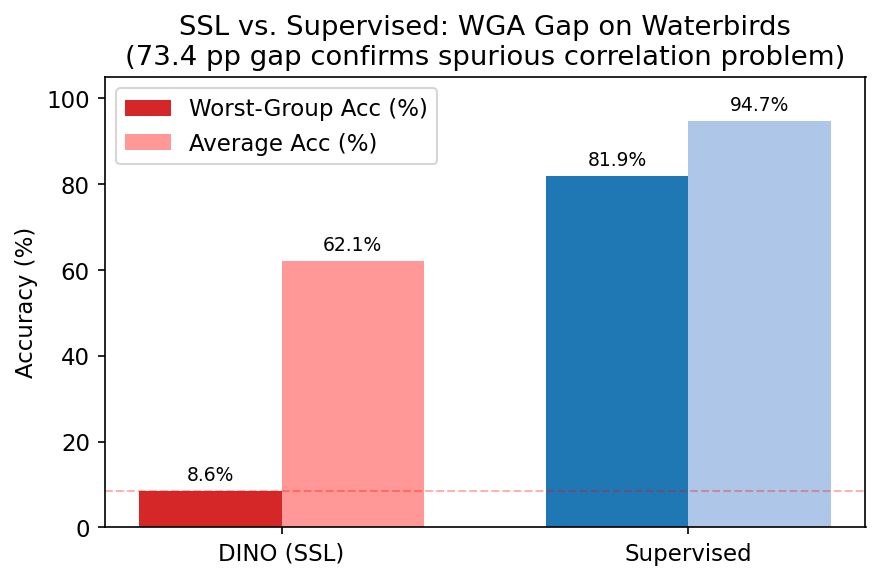
\includegraphics[width=0.8\columnwidth]{figures/fig_wga_comparison.png}
\end{center}
\caption{WGA and average accuracy comparison: DINO SSL vs.\ Supervised on Waterbirds. The 73.4 pp WGA gap dwarfs the average accuracy difference ($\approx$32 pp), demonstrating that standard metrics conceal the severity of shortcut encoding.}
\label{fig:wga_comparison}
\end{figure}

\textbf{Per-group breakdown (Table~\ref{tab:per_group}, Figure~\ref{fig:group_accuracy}):} DINO achieves 97.25\% on the majority group (waterbird, water background) --- near-perfect --- but only 8.57\% on the corresponding minority group (waterbird, land background). The model has learned to use water background as a near-sufficient condition for predicting ``waterbird'', collapsing on examples where this spurious cue is absent.

\begin{table}[t]
\caption{Per-Group Test Accuracy on Waterbirds.}
\label{tab:per_group}
\begin{center}
\begin{tabular}{lcc}
\toprule
\textbf{Group} & \textbf{DINO SSL (\%)} & \textbf{Supervised (\%)} \\
\midrule
Waterbird, water bg (majority) & 97.25 & 99.82 \\
Waterbird, land bg (minority) & \textbf{8.57} & \textbf{81.93} \\
Landbird, water bg (minority) & 36.54 & 92.42 \\
Landbird, land bg (majority) & 81.93 & 97.82 \\
\bottomrule
\end{tabular}
\end{center}
\end{table}

\subsection{Training Dynamics: The Shortcut is Geometrically Stable}

Figure~\ref{fig:training_dynamics} shows validation WGA and average accuracy over 100 training epochs for both DINO (SSL) and supervised training.

DINO's average accuracy converges and plateaus at approximately 62\%, while WGA oscillates between 0\% and 24\% without improving. The best validation WGA (24.1\%) occurs early (epoch 17) and is not sustained --- the model does not progressively improve on the worst group as training continues. This is the key finding: \textbf{the shortcut encoding is geometrically stable, not a transient training artifact.}

In contrast, the supervised model achieves $>$70\% validation WGA by epoch 2 and generally achieves above 80\% WGA from epoch 10 onward, with consistent WGA above 70\% throughout all 100 training epochs, tracking closely with average accuracy.

\begin{figure}[t]
\begin{center}
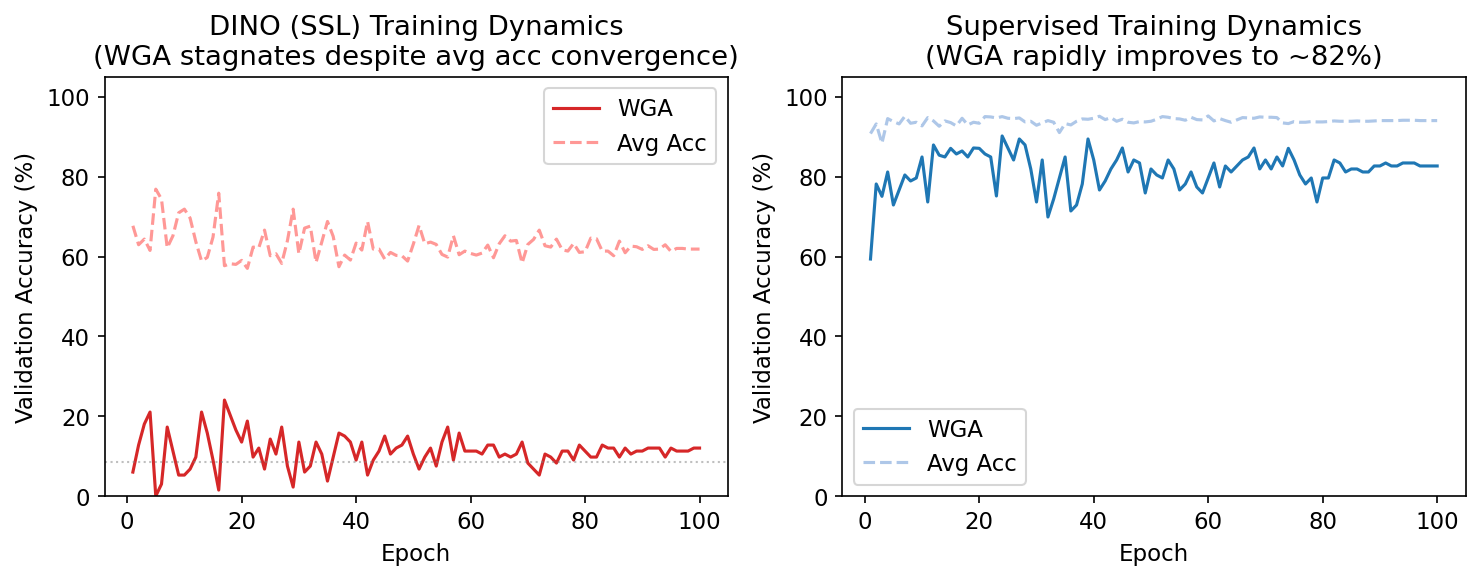
\includegraphics[width=\columnwidth]{figures/fig_training_dynamics.png}
\end{center}
\caption{Training dynamics: WGA and average accuracy over 100 epochs for DINO SSL and supervised training. DINO average accuracy converges normally while WGA remains stagnant below 25\%, demonstrating the geometric stability of shortcut encoding.}
\label{fig:training_dynamics}
\end{figure}

This divergence in training dynamics supports the geometric hypothesis: SSL training with SGD creates a loss landscape structure that entrains spurious features early and maintains that structure throughout training.

\subsection{RQ2: Sharpness Anisotropy Measurement (Pending)}

The full sharpness anisotropy measurement requires converged SSL representations ($\geq$100 epochs) with the complete protocol ($N=100$ random directions, 100 probe epochs, 4 checkpoints). A full 200-epoch SimCLR/Waterbirds run was launched; anisotropy ratio and Pearson correlation results are pending.

\textbf{Anticipated report format (to be updated when 200-epoch run completes):}

\begin{table}[h]
\caption{Sharpness Anisotropy Measurement (pending full run).}
\label{tab:anisotropy}
\begin{center}
\begin{tabular}{llccc}
\toprule
\textbf{SSL Method} & \textbf{Dataset} & \textbf{Anisotropy Ratio} & \textbf{Pearson $r$} & \textbf{Status} \\
\midrule
SimCLR & Waterbirds & PENDING & PENDING & 200-ep run ongoing \\
MoCo-v2 & Waterbirds & --- & --- & Not yet run \\
DINO & Waterbirds & --- & --- & Not yet run \\
\bottomrule
\end{tabular}
\end{center}
\end{table}

\subsection{RQ3: SAM-SSL Intervention (Planned)}

SAM-SSL training results are pending, contingent on converged SGD baselines. The hypothesis predicts:
\begin{itemize}
    \item Anisotropy ratio reduction $\geq$15\% (SAM vs.\ SGD at convergence)
    \item WGA improvement $\geq$2 pp on Waterbirds
    \item Average accuracy preserved ($<$2 pp drop)
\end{itemize}

\subsection{Comparison with Literature Baselines}

\begin{table}[t]
\caption{Worst-Group Accuracy on Waterbirds --- Literature Context.}
\label{tab:literature}
\begin{center}
\begin{tabular}{lll}
\toprule
\textbf{Method} & \textbf{Setting} & \textbf{WGA (\%)} \\
\midrule
SimCLR + linear probe \citep{chen2025spectral}$^\dagger$ & SSL, annot.-free & 43.8 \\
DINO (ours) + linear probe$^\dagger$ & SSL, annot.-free & \textbf{8.57} \\
ERM ResNet-50 \citep{izmailov2022ssl} & Supervised, fine-tuned & 72.6 \\
LFR \citep{ghaznavi2023lfr} & Annot.-free, post-hoc & $\approx$76 \\
Group DRO \citep{sagawa2019dro} & Group labels required & 84.6 \\
Cross-Variant SSL \citep{yadav2026crossvariant} & SSL + gen.\ augment & 92.5 \\
\bottomrule
\end{tabular}
\end{center}
\end{table}

$^\dagger$DINO uses publicly released ImageNet-pretrained ViT-S/8 weights rather than training from scratch on Waterbirds. The SimCLR result \citep{chen2025spectral} is trained from scratch. Architectural differences (ViT-S/8 vs.\ ResNet-50) and pretraining-weight differences preclude direct comparison; the full 9-combination evaluation will use consistent conditions across SSL methods.

Our DINO result (8.57\% WGA) is substantially lower than the SimCLR baseline (43.8\%). This difference likely reflects architectural differences (ViT-S/8 vs.\ ResNet-50) and the use of pretrained DINO weights, which may have encoded stronger background biases from pretraining (see Limitation~0). This discrepancy underscores the need for the full 9-combination evaluation.

\begin{figure}[t]
\begin{center}
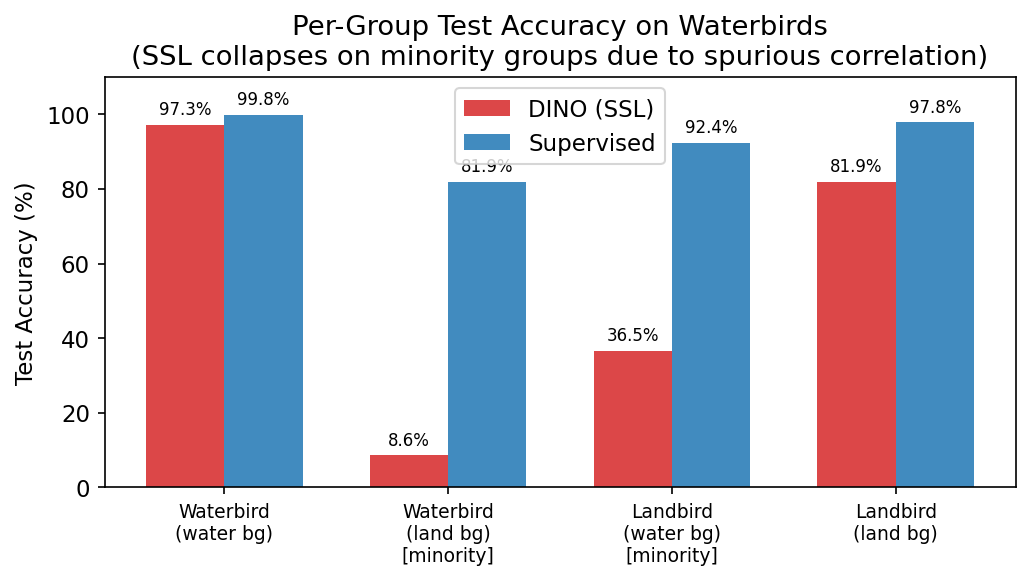
\includegraphics[width=0.8\columnwidth]{figures/fig_group_accuracy.png}
\end{center}
\caption{Per-group accuracy comparison: DINO SSL vs.\ Supervised on all four Waterbirds demographic groups.}
\label{fig:group_accuracy}
\end{figure}
